\section{Conventions de représentations}

\subsection{Présentation de la convention retenue}
L'algorithme prend un graphe dirigé en entrée et retourne un booléen, qui indique si le graphe possède un cycle ou non. Il nous faut donc définir une convention de représentation d'un graphe dirigé sur lequel notre algorithme va s'appliquer. \\

Le graphe sera représenté en utilisant des listes d'adjacence (adjacency list structure). Dans cette structure, chaque objet noeud contient une référence vers la liste des arêtes qui sortent de celui-ci (mais pas celles entrantes). De même, chaque objet arête, contient une référence au noeud vers lequel elle se dirige. La Figure~\ref{schéma} illustre cette structure dans le cas d'un graphe non dirigé où $V$ est l'ensemble des sommets $I(v)$ représente la liste des arêtes adjacentes au noeud $v$ et $E$ est l'ensemble des arêtes. Nous adaptons un peu ce schéma pour le cas d'un graphe dirigé sur lequel on appliquera notre algorithme en disant qu'un noeud ne doit connaître que la liste des arêtes sortantes et qu'une arête ne doit connaitre que sa destination. Nous ajoutons également à la classe noeud une variable d'instance incounter comptant le nombre d'arêtes entrantes au noeud. 

\begin{figure}[!h]
	\centering
         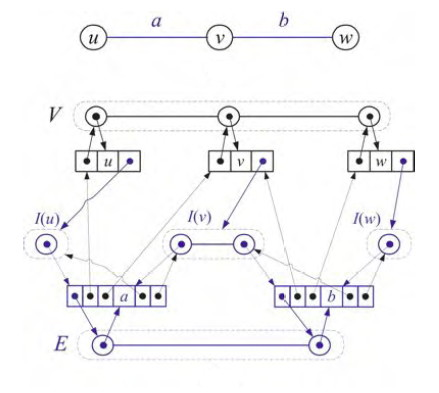
\includegraphics[width=0.5\textwidth]{1convderepr/schema.jpg}
         \label{schéma}
         \caption{Liste d'adjacence}
\end{figure}

\subsection{Motivations}
Le fait de représenter un graphe avec la structure décrite précédemment possède divers avantages. Ceux-ci sont les suivants : \\

\begin{itemize}
\item \textbf{Facilité d'implémentation} : dans l'algorithme à implémenter, les actions principales à effectuer sur le graphe sont de trouver les arêtes sortantes d'un noeud, les noeuds vers lesquels elles se dirigent et de diminuer leur incounter. L'implémentation de ces deux fonctionnalités est très facile car chaque objet contient les références nécessaires.

\item \textbf{Complexité satisfaisante} : nous prouverons plus tard que la complexité temporelle de l'algorithme avec notre structure de données est en $\mathcal{O}(n + m)$ où $n$ et $m$ sont respectivement le nombre de noeud et d'arêtes du graphe. Nous ne pourrions pas faire mieux étant donné qu'il va au pire effectivement falloir passer par tous les noeuds et les arêtes. Deux autres représentations de graphe existent : la edge list structure et la adjacency matrix structure. La première a une complexité en $\mathcal{O}(m)$ pour trouver les arêtes adjacentes à un sommet alors qu'avec notre structure la complexité est en $\mathcal{O}(1)$. La matrice d'adjacence présente aussi des désavantages à ce niveau là car passer par toutes les arêtes est en $\mathcal{O}(n^2)$ au lieu de $\mathcal{O}(m)$.
\end{itemize}
